\section{Code setup}
\label{sec:setup}
In order to implement the models to be solved we decided to use the common and powerful tool \href{https://www.ibm.com/products/ilog-cplex-optimization-studio}{IBM CPLEX}. Usually this software isn't free but due the academic usage it was made available for all the students that needed it.\\
CPLEX allow its user to decide which programming language to use between Python and C; in this project we used C.

To visualize the nodes and the paths found by our program we used a \href{https://www.gnuplot.info}{Gnuplot} which is a command-line driven utility. Its code is protected byt copyright but the download is completely free. The sofware needs to be installed on the machine where the code is executed because Gnuplot is executed as a pipe: in particular before the plotting all the data is wrote to a file (according to the documentation) and than Gnuplot read and create the plot from that file.

To build the performance profiles in this report we used a python program written by D. Salvagnin (2019).


The first thing we did was build a parser capable of interpreting the TSP problems provided by the \href{http://comopt.ifi.uni-heidelberg.de/software/TSPLIB95/}{TSPLIB}. The main data to save was the number of nodes, the coordinates of the nodes (they will be or relative coordinates that describe the position of the nodes or real world coordinates), the type of distance function to use (for example when are used real world coordinates the distance function need to consider the sphericity of the world). For each tsp problem we assume that the datafile contains a complete graph, so each node is directly connected with all the others nodes.

In my particular case all the project was developed on a linux machine with Ubuntu 20.04.

\subsection{CPLEX environment}
\label{cap:2_int}
In order to work properly CPLEX needs to build his internal data structure to hold all the information needed to solve the problem. So the first thing to do is to create a pointer to the environment of Cplex through the \verb|CPXopenCPLEX(&error)|: this function will return a pointer to the CPLEX environment that will be needed to use his entire library.\\
Once the environment is build CPLEX needs an additional data structure to hold the constraints of the optimization problem we want to solve, in order to use it we build an empty object using the function \verb|CPXcreateprob(env, &error, "TSP")|: this will return a pointer to the problem where we will write all the constraints that we need.

\begin{lstlisting}
CPXENVptr env = CPXopenCPLEX(&error);
CPXLPptr lp = CPXcreateprob(env, &error, "TSP");
\end{lstlisting}

\subsubsection{Variable and constraint creation}
Now that the enviroment is setted up we can start by creating our first variable. CPLEX handle the variable and constraints respectivetely as columns and rows; to unserstand it better let's make an example with a simple minization problem:

\[ \begin{array}{lllllll}%
	\text{min}  &x_1 	&+ 	& 3x_2 &+ & x_3\\
	  			&  2x_1 &  	&   &- &x_3 &\le 60\\
	  			&		&	& 4x_2 & + &7x_3 &\ge 20\\
\end{array}\]%
\begin{align*}
x_i \; \text{integer}\
\end{align*}

Thius problem can be seen as a matrix composed by rows and columns, each column correspond to a variable, each row correspond to a constraint that the problem as to satisfy. Using the callable library of CPLEX we can build the rows and columns easily.\\
To build the variable we need to add a column to the problem, we can to this using the method \verb|CPXnewcols|; this method allow us to create more than a single column per time through his parameters, in our case we built each variable singularly as shown in the code:

\begin{lstlisting}
	CPXnewcols(env, lp, 1, &obj, &lb, &ub, &variable_type, cname)
\end{lstlisting}

Here \verb|env| and \verb|lp| are respectively the  pointers toi the environment and to the problem build in the section \ref{cap:2_int}.
The arguments \verb|&obj, &lb, &ub, &variable_type, cname| are arrays that contains the values for the objective function, lower bound, upper bound, variable type and name for each variable. The last argument to analyze is the number $1$, it represent the number of variables to add during this call to the CPLEX's library (as said before in this project we build the variables singularly).

At the end of this phase we have only the variable used in the objective function, now we will discuss how the constraints are implemented in the code. This time the process is more complicated that the previous one, in fact we need first to build an empty constraint, that means that on the left side there are no variables or numbers, than we change the coefficients for each variable. Let's explain it with and example:

\begin{lstlisting}
	CPXnewrows(env, lp, 1, &rhs, &sense, NULL, cname)
\end{lstlisting}

Here \verb|env, lp, 1| and \verb|cname| corresponds at the same variable as in the case of the columns, \verb|&rhs| is the righthand side term for each constraint to be added to the problem object, \verb|&sense| is the sense of each constraint to be added to the problem object, \verb|NULL| contains the range values for the new constraints, for example it sets a maximum/minimum value to each constraint.\\
At this point we have something like this (example with random values):
\[ \text{*empty*} \qquad \le 30\]
So a part of the constraint is build, we need to decide what variables we want to put in this inequation. In order to do that we use the function \verb|CPXchgcoef|. 

Before seeing this method in detail we will explain how CPLEX reference to the rows and columns. In fact the name that we pass to the callable library are not directely used by CPLEX but are needed to the developer to understand if the problem is built correctely; for its function CPLEX simply enumerates each row and each column, so if we want to reference to a specific variable or constraint we need to now its number; by creating variables and constraint we know exactely which is built before and whic after, so for example in the optimization problem shown at the begginning of the section to $x_1$ is given the number 1, to $x_2$ the number 2 and so on. The same thing happens to the constraints. Now we can fully understand the method previously introduced.

\verb|CPXchgcoef| uses the already known arguments \verb|env| and \verb|lp|, in addition to them in needs the number of the constraint we want to modify, the number of the variable we want to change the coefficent and the coefficient for that variable. For example to build the first contraint of the already used optimization problem we need two calls to this method since we need to modify two coefficients of the variables:

\begin{lstlisting}
	// Here the first number is the id of the constraint
	// the second is the id of the variable (1 for x1, 3 for x3)
	// and the third one id the value of the coefficents
	// (2 for x1 and -1 for x2)
	CPXchgcoef(env, lp, 1, 1, 2.0);
	CPXchgcoef(env, lp, 1, 3, -1.0);
\end{lstlisting}

Now that we have introduced the code setup and how the models are built we can start by examinating the variuos methods that we have use to solve the TSP optimization problem.

\subsection{Solution and data management}
\label{sec:sol_management}
In this section we will explain how we managed the data from the .tsp file and how we handled the solution obtained with CPLEX.

The first thing we build was a new struct that contains all useful data read from the .tsp file provided by the TSPLIB. Theese files in fact contains different infromations:

\begin{itemize}
	\item NAME: the name of the file;
	\item COMMENT: some comment on the data;
	\item TYPE: the type of the problem;
	\item DIMENSION: the number of nodes that are in the file;
	\item EDGE\_WEIGHT\_TYPE: the typology of the distance between the nodes;
	\item NODE\_COORD\_SECTION: section, usally it goes to the end of the file, in which are described the nodes coordinates.
\end{itemize}

We decided to save only the fundamentals informations, in our case only the number of nodes, the node coordinates and the type of the distance functions between the nodes. All these data are saved into the struct during the parsing operation of the .tsp file.

After the solution is computed by CPLEX we can access it by using the method \verb|CPXgetx|. This function will return the full array of variables, than by checking their values (1 if is true) we can see if some edge has been selected and if it is valid we save it to an array inside our struct.

Now we have our solution saved its time to check if it is a single tour or if there are sub-tours. To do that we use a simple trick, since the edges are connected with two nodes, we start from the first edge extracted and we go to one of the nodes, now we are there we check at what node this one is connected. If we already visited the next node we end our cycle and we continue the algorithm by checking all the unvisited nodes, if there is any.\\
To save each subtour we use and additional array that will contain the tour number at which each node belong, see figure \ref{img:comp} for a graphical representation.

\begin{figure}
	\centering
	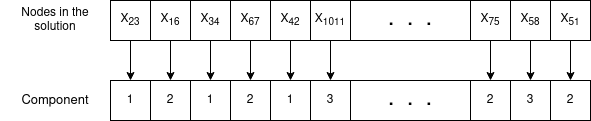
\includegraphics[width=0.8\textwidth]{images/components}
	\caption{Structure of the solution. Each variable extracted from the solution provided by CPLEX is associated with a number that specify in which tour the variable belongs. In case of a solution with one tour all the array component will be filled with 1's.}
	\label{img:comp}
\end{figure} 